% Figure pour illustrer que si deux ouverts sont disjoints, alors
% l'adhérence du premier est disjoint du second ouvert
\begin{figure}[!h]
  \begin{center}
    \caption{Illustration du lemme \ref{rap:top1}}%
    \label{fig:ouv_disjoints}
    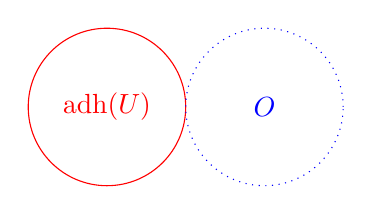
\begin{tikzpicture}
      \draw [red] (0 , 1) ellipse (1 cm and 1 cm) node {$\mathrm{adh}(U)$};
      \draw [blue, dotted] (2 , 1) ellipse (1 cm and 1 cm) node {$O$};
    \end{tikzpicture}
\end{center}
\end{figure}
